\documentclass[12pt]{article}
\usepackage[portuguese, brazilian, english]{babel}
\usepackage[utf8]{inputenc}
\usepackage[usenames,dvipsnames]{color}
\usepackage{setspace}
\usepackage{amsmath}
\usepackage{amsfonts}
\usepackage{amssymb}
\usepackage{mathtools}
\usepackage[top=3cm, bottom=2cm, left=3cm, right=2cm]{geometry}
\usepackage{tikz}
\usepackage{textcomp}
\usepackage{lscape}    % for landscape pages
\usepackage{hyperref}  % to allow hyperlinks
\usepackage{booktabs}  % nicer table borders
\usepackage{graphicx, subfigure} % add subfigures
\usepackage{rotating}  % sideways figure
\usepackage[verbose]{placeins} % avoids placing figures on last page
\usepackage{fullpage}

\mathchardef\myhyphen="2D  % define hyphenation in math mode
                          % (useful for enzyme--substrate complex notation)


\title{Projeto MSc}

% Figures directory
\graphicspath{{./figures/}} 

\definecolor{myblue}{RGB}{80,80,160}
\definecolor{mygreen}{RGB}{80,160,80}
\setstretch{1.5}

\begin{document}

% FAPESP demands the usage of double spacing
%
\doublespacing

\selectlanguage{brazilian}
\thispagestyle{empty} 
\begin{flushright}
    {\LARGE Identificação de vias de sinalização celular baseada em repositórios de cinética de reações bioquímicas}

  {\large {\bf Bolsista:} \href{mailto:gustavo.estrela.matos@usp.br}{Gustavo Estrela de Matos}\\ 
    {\bf Orientador:} \href{mailto:marcelo.reis@butantan.gov.br}{Marcelo da Silva Reis}}\\
  {\small Centro de Toxinas, Imuno-resposta e Sinalização Celular (CeTICS)\\
     Laboratório Especial de Ciclo Celular (LECC)}\\
  Instituto Butantan, São Paulo, \today.\\

\end{flushright}
\begin{abstract}
    
A construção de modelos funcionais é uma técnica comum para se 
estudar vias de sinalização celular e, quando a via estudada é pouco
conhecida, é possível que os modelos já propostos sejam incompletos, 
tornando necessário a sua modificação.
Lulu Wu apresentou em 2015, em sua dissertação de mestrado, um método 
para  modificar sistematicamente modelos funcionais, adicionando a estes
interações extraídas de repositórios como KEGG. Entretanto, esta 
metodologia apresentou limitações: a primeira é a incompletude do banco 
de dados de interações criado, que extraia informações apenas do 
repositório KEGG; a segunda, a falta de informações sobre constantes 
de velocidade de interações, que podem ser extraídas de repositórios 
como BioNumbers; a terceira, a dinâmica do algoritmo de busca, 
incremental, que pode não achar o mínimo global; e a última, a 
penalização na complexidade dos modelos, que era feita de maneira 
aleatória. Propomos neste trabalho enfrentar as limitações encontradas
pela metodologia de Lulu, criando um banco de dados de interações mais
completo e também novas funções de custo que sejam capazes de 
penalizar modelos mais complexos (como critério de informação Akaike e 
{\em Bayesian inference-based modeling}); esta penalização deve induzir,
em cadeias do  espaço de busca, curvas em u no custo dos modelos, 
portanto também propomos a criação de novos algoritmos de busca que 
explorem essa característica da função de custo. Por fim, esperamos 
testar nossa metodologia na identificação de vias de sinalização celular 
da linhagem tumoral murina Y1.
\end{abstract}

\newpage
\thispagestyle{empty} 
\selectlanguage{english}
\begin{flushright}
    {\LARGE Identification of cell signaling pathways based on biochemical reaction kinetics repositories}

    {\large {\bf Student:} \href{mailto:gustavo.estrela.matos@usp.br}{Gustavo Estrela de Matos}\\ 
    {\bf Supervisor:} \href{mailto:marcelo.reis@butantan.gov.br}{Marcelo da Silva Reis}}\\
    {\small Center of Toxins, Immune-response and Cell Signaling (CeTICS)\\
    Laboratório Especial de Ciclo Celular (LECC)}\\
  Instituto Butantan, São Paulo, \today.\\
\end{flushright}
\begin{abstract}
It is usual to create computational models to study cell signaling 
pathways and, when this pathway is not well known, it's possible that 
currently proposed models are incomplete, making it necessary to make 
modifications on the model. Lulu Wu presented in 2015, on her master's 
dissertation, a method for systematically modifying models, adding to 
them interactions extracted from repositories such as KEGG. However, 
this method showed some limitations: the first is the interactions
database incompleteness, which extracted informations from KEGG database
only; the second, the lack of information about interactions rate 
constants, what could be gathered from repositories such as BioNumbers; 
the third, the dynamics of the search algorithm, incremental, that might 
not find the global minimum; and finally, the cost function penalization 
on model complexity, which was aleatory. We propose on this project to 
confront the limitations presented on Lulu's methodology, creating a
more complete interaction database and also new cost functions that are 
able to penalize more complex models (such as the Akaike information
criteria and Bayesian inference-based modeling); this penalization is 
likely to induce, on chains of the search space, u shaped curves on 
model costs, therefore we also propose new search algorithms that 
explore this feature of the cost function. Finally, we expect to use our
methodology on identification of cell signaling pathways of the murina 
Y1 tumoral cell line.
\end{abstract}

\newpage
\selectlanguage{brazilian}
\tableofcontents
\newpage

\section{Introdução}

A sinalização celular é um processo de troca de informações que ocorre no interior de uma célula e em suas imediações por meio de interações entre espécies químicas. Um conjunto de interações que estão associadas a uma determinada transmissão de informação (e.g., um sinal que chega no núcleo celular a partir do acionamento de um receptor de membrana citoplasmática) é chamado de via de sinalização celular.
Diversos processos celulares são coordenados por vias de sinalização celular; por exemplo, o ciclo celular pode ser estimulado a partir de uma sinalização mitogênica, que trafega por algumas dessas vias (e.g., pelas vias das \href{https://en.wikipedia.org/wiki/Mitogen-activated\_protein\_kinase}{MAP quinases}). Portanto, entender a topologia e a dinâmica dessas vias pode ajudar a elucidar o funcionamento de diversos tipos de células. Ademais, uma vez que anomalias em vias de sinalização celular podem levar ao desenvolvimento de doenças tais como o câncer e o diabetes, desvendar propriedades de seus mecanismos é uma etapa inicial, porém altamente relevante, no desenvolvimento de novos tratamentos contra essas doenças.

O estudo de uma via de sinalização é realizado através da observação, ao longo de uma determinada janela de tempo, da concentração de algumas das espécies químicas envolvidas no fenômeno. Dependendo do contexto, a via de sinalização pode ser estudada com a aplicação de testes estatísticos e de análises de correlações sobre resultados dos experimentos biológicos. Todavia, como geralmente é possível medir apenas alguns instantes de tempo de uma fração das espécies químicas envolvidas, faz-se necessário agregar nessas análises informações {\em a priori} vindas do conhecimento existente da cinética de reações bioquímicas, o que pode ser feito com modelos dinâmicos computacionais. 

Um tipo particular de modelo dinâmico computacional, denominado modelo funcional, pode descrever a concentração de espécies químicas ao longo do tempo, através de algum formalismo matemático das regras definidas pela cinética de reações bioquímicas; por exemplo, empregando sistemas de equações diferenciais ordinárias (EDOs). Os modelos funcionais, quando corretamente definidos, são capazes de simular o que pode ser observado por experimentos biológicos. Além de incorporar às análises informações {\em a priori} relevantes, o uso desse tipo de modelo também traz a vantagem de ser uma abordagem \underline{preditiva}: considerando que o modelo desenhado aproxima bem a realidade e que não padece de {\em overfitting}, o mesmo pode prever a dinâmica da via de sinalização para diferentes estados (condições) iniciais. Isso pode ser utilizado, por exemplo, para testar o comportamento de uma via de sinalização celular de acordo com o tratamento dado às células.

Portanto, o desenho de modelos funcionais para o estudo de vias de sinalização celular é um problema relevante no contexto de Biologia Celular Molecular e de Biomedicina; uma definição desse problema, bem como métodos para abordá-lo, serão apresentados a seguir.

\subsection{Identificação de vias de sinalização celular}
O problema de desenhar modelos funcionais, que sejam capazes de explicar os resultados obtidos em experimentos biológicos e que ao mesmo tempo minimizem o problema de {\em overfitting}, é chamado de {\em problema de identificação de vias de sinalização celular}. Tipicamente, a resolução desse problema é realizada em duas etapas: na primeira delas, escolhemos as espécies químicas e interações que participam da via, definindo assim as EDOs que farão a descrição matemática da dinâmica do modelo ao longo de uma determinada janela de tempo. Já na segunda etapa, são determinados valores para as constantes de velocidade (i.e., os valores dos parâmetros do sistema de EDOs) e também para as concentrações iniciais (i.e., o estado inicial do modelo dinâmico); se não é possível encontrar valores adequados para os parâmetros, então é preciso voltar para a primeira etapa e redefinir as espécies químicas e/ou interações envolvidas.

Para a resolução da primeira etapa, frequentemente recorre-se a interações entre espécies químicas listadas em bancos de dados de interatomas tais como o \href{http://www.genome.jp/kegg/}{Kyoto Encyclopedia of} \href{http://www.genome.jp/kegg/}{Genes and Genomes (KEGG)}~\cite{Kanehisa2000kegg}. KEGG e outros bancos de dados similares apresentam uma vasta coleção de interatomas (também conhecidos como mapas estáticos), catalogados por organismo, tipo de tecido, via de sinalização estudada, etc. Logo, o pesquisador normalmente recorre ao mapa cuja categoria mais se aproxime das condições de seu experimento biológico para selecionar as interações que comporão seu modelo funcional. Outra alternativa é recorrer a um modelo {\em scaffolding} para servir de base ao modelo funcional em desenvolvimento, para este fim recorrendo a bancos de dados de modelos; um exemplo desse tipo de banco de dados é o \href{https://www.ebi.ac.uk/biomodels-main/}{BioModels}~\cite{le2006biomodels}.

Já para a segunda etapa, é possível utilizar constantes de velocidade disponíveis na literatura e/ou em bancos de dados tal como o \href{http://bionumbers.hms.harvard.edu/}{BioNumbers}~\cite{milo2009bionumbers}, que são determinadas através de experimentos biológicos (e.g., em \href{https://en.wikipedia.org/wiki/Enzyme\_assay}{ensaios enzimáticos}). Quando tais constantes não estão disponíveis, precisamos recorrer a um método conhecido como \href{https://en.wikipedia.org/wiki/Curve\_fitting}{otimização por ajuste de curva} (do inglês \emph{curve-fitting optimization}). Nesse tipo de otimização, para um dado conjunto de valores para os parâmetros do modelo funcional, uma simulação é realizada e seu resultado é comparado com os dados coletados experimentalmente, segundo uma dada medida de erro (i.e., a função custo); com a ajuda de um algoritmo de otimização, tal procedimento é realizado muitas vezes, até que algum critério de parada seja atingido (e.g., um limiar superior para o erro). Uma opção de ferramenta para a realização de otimização por ajuste de curva é o \href{https://github.com/vincent-noel/SigNetSim}{Signaling Network Simulator (SigNetSim)}.

Um exemplo de resolução do problema de identificação de vias de sinalização celular é mostrado na figura~\ref{fig:example_reis_interdisciplinary}, no qual é realizada uma primeira iteração da primeira e segunda etapas (figuras~\ref{fig:example_reis_interdisciplinary:A} e \ref{fig:example_reis_interdisciplinary:B}) que não foi capaz de explicar as medidas dos experimentos biológicos; dessa forma, foi realizada uma segunda iteração dessas duas etapas (figuras~\ref{fig:example_reis_interdisciplinary:C} e \ref{fig:example_reis_interdisciplinary:D}), com resultados muito mais satisfatórios.

\begin{figure}[h]
    \begin{tabular}{ll}
        \centering
    \subfigure[] {
        \label{fig:example_reis_interdisciplinary:A}
        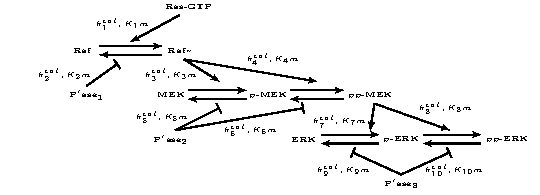
\includegraphics[trim = 0.5cm 0cm 0cm 0cm, clip=true, width=0.5\textwidth]{Figure_3.pdf}
    }
    &
    \subfigure[] {
        \label{fig:example_reis_interdisciplinary:B}
        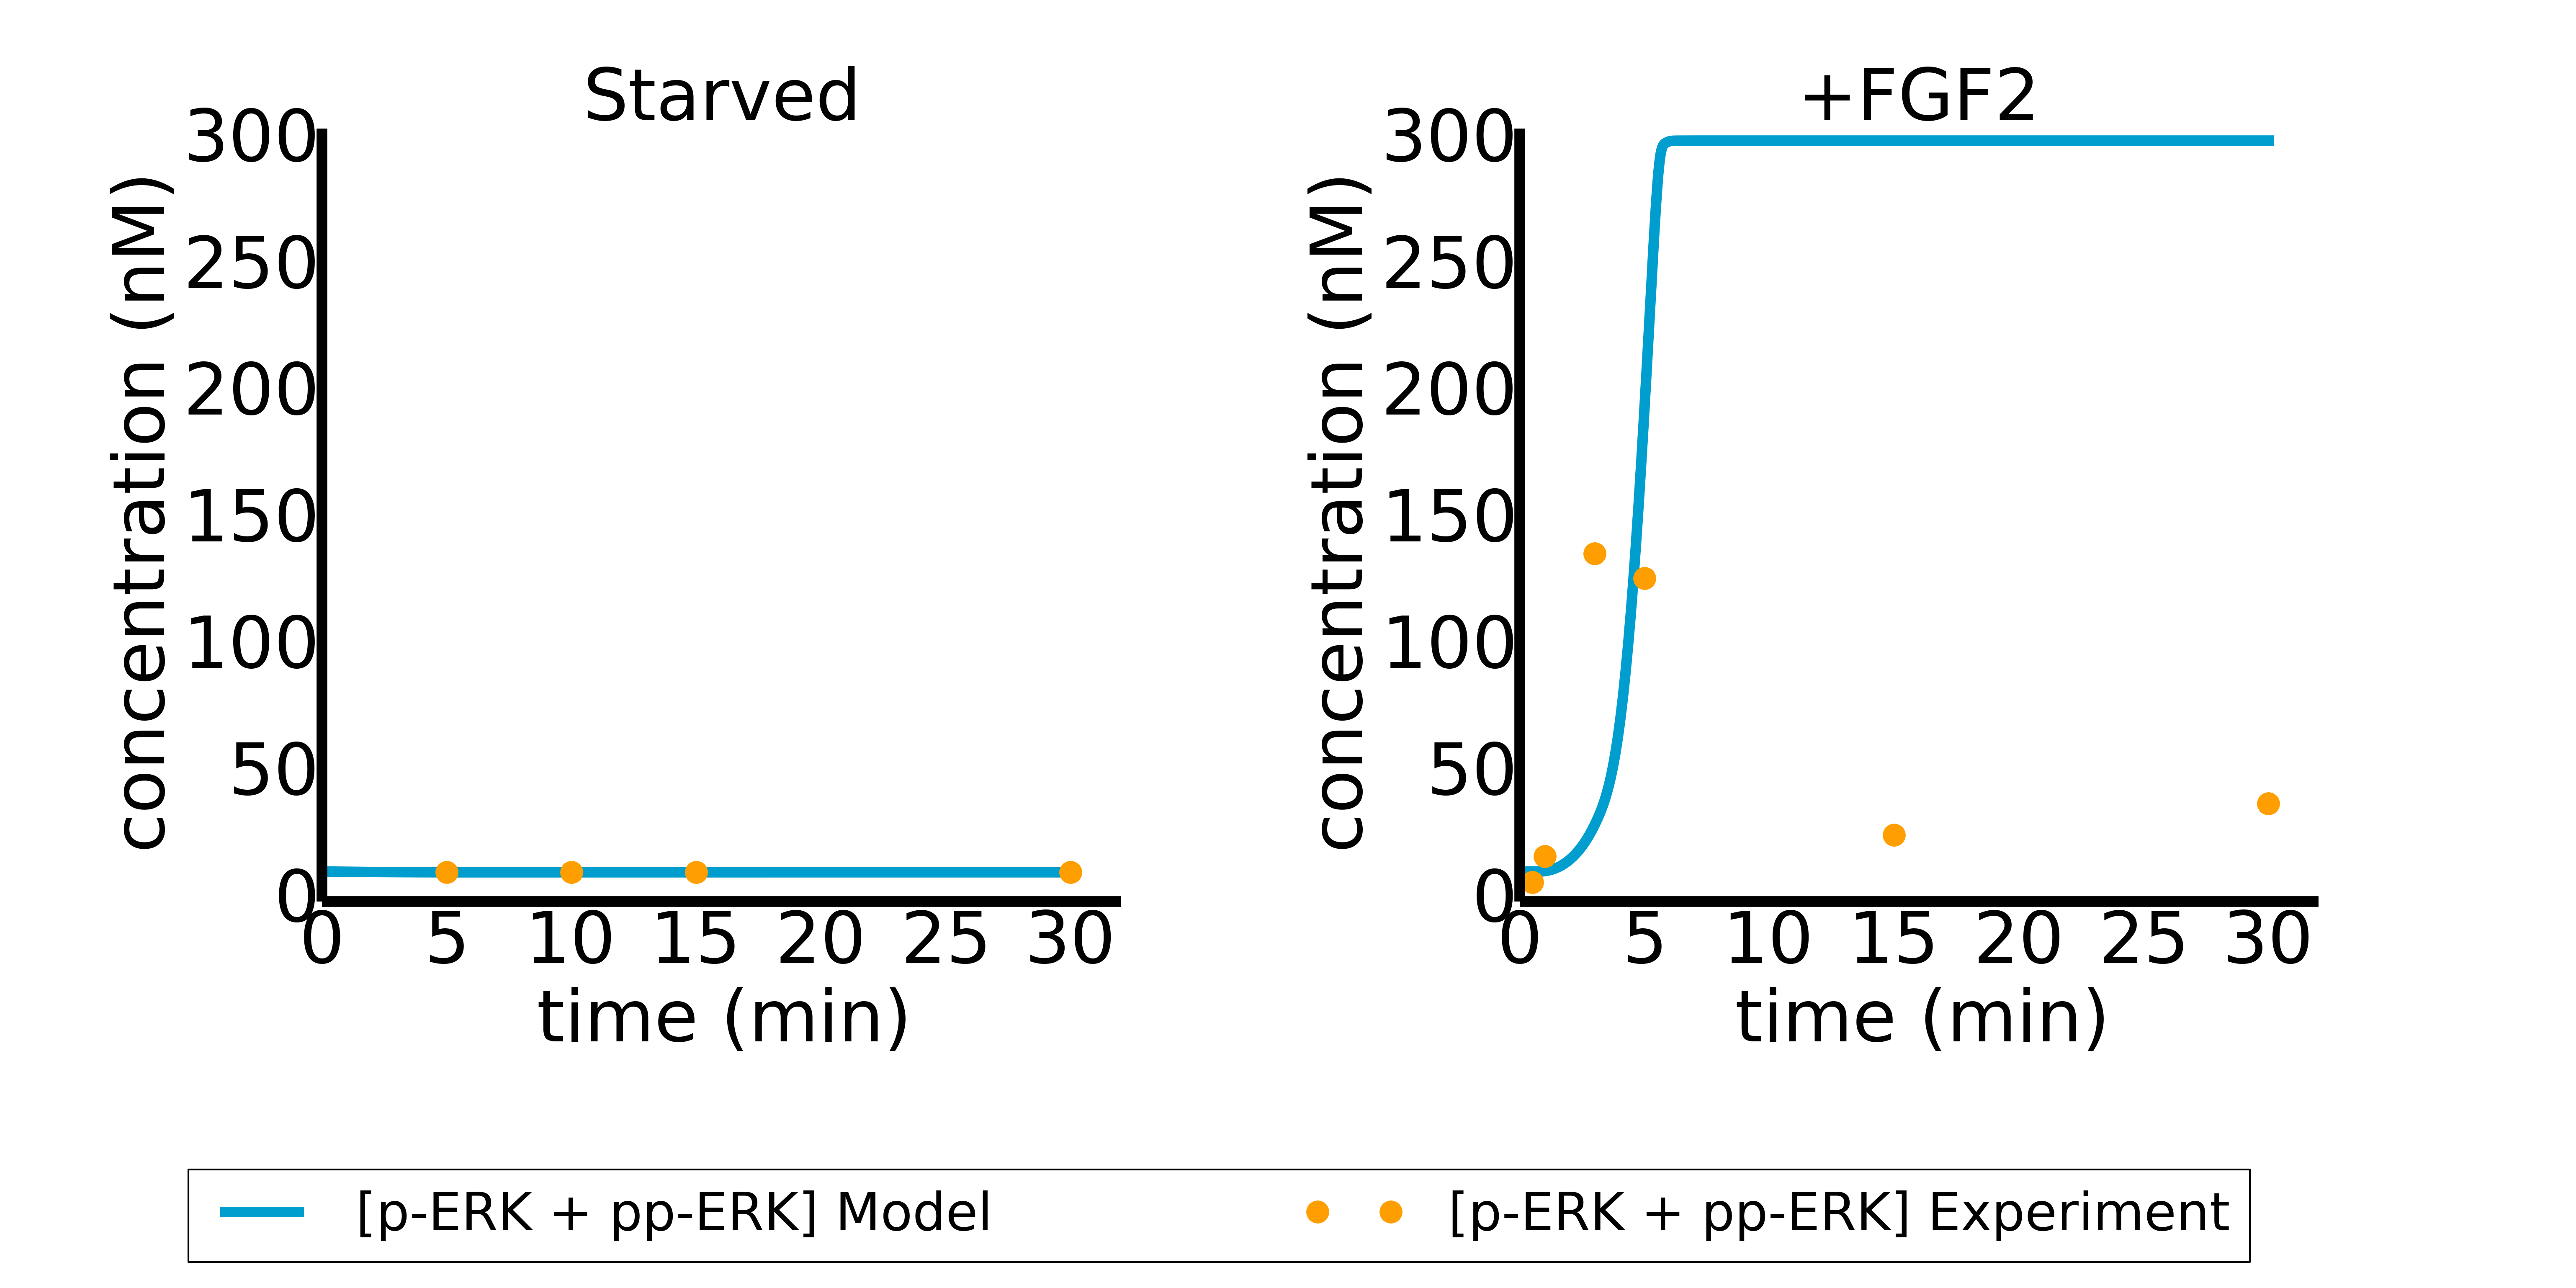
\includegraphics[trim = 0.5cm 0cm 0cm 0cm,clip=true, width=0.5\textwidth]{Figure_5.png}
    }
    \\
    \subfigure[] {
        \label{fig:example_reis_interdisciplinary:C}
        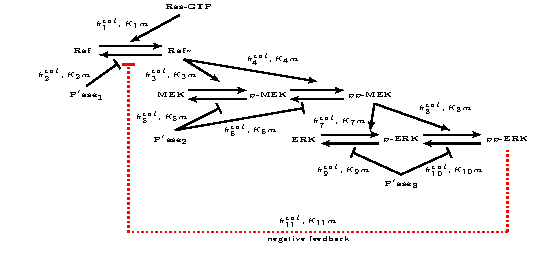
\includegraphics[trim = 0.5cm 0cm 0cm 0cm, clip=true, width=0.5\textwidth]{Figure_6.pdf}
    }
    &
    \subfigure[] {
        \label{fig:example_reis_interdisciplinary:D}
        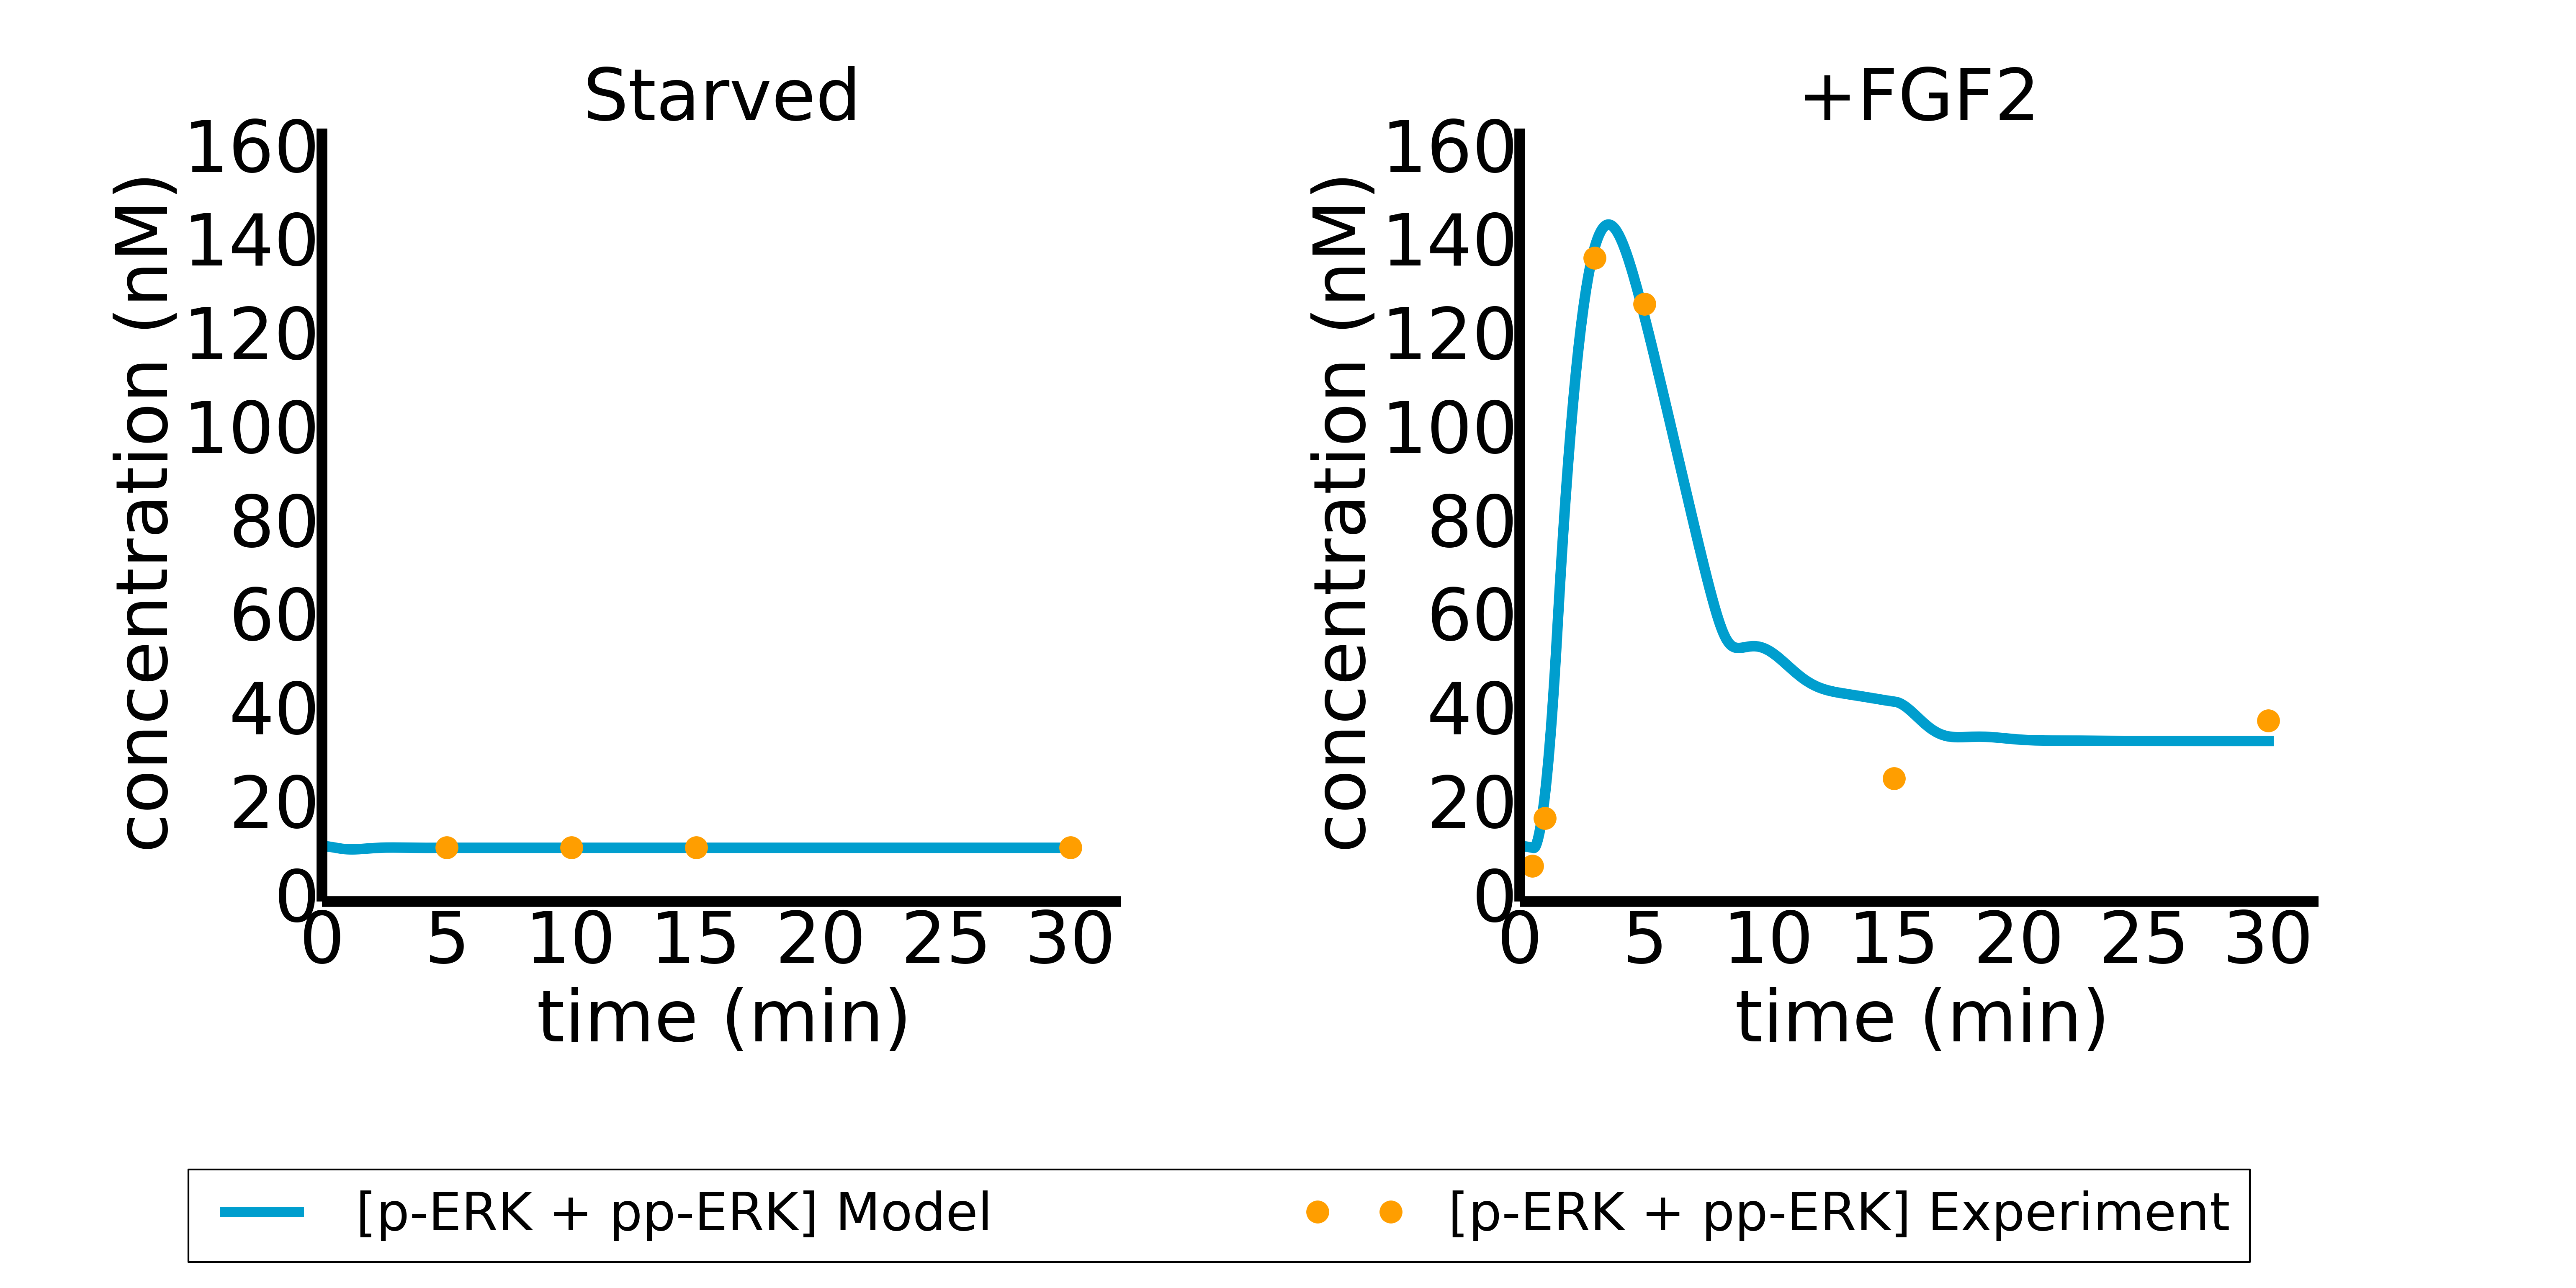
\includegraphics[trim = 0.5cm 0cm 0cm 0cm,clip=true, width=0.5\textwidth]{Figure_7.png}
    }
    \end{tabular}   
    \caption{Exemplo de identificação da via de sinalização Ras/ERK em células murinas de carcinoma adrenocortical Y1, conforme apresentado em Reis e colegas~\cite{Reis2017interdisciplinary}. As figuras~\ref{fig:example_reis_interdisciplinary:A} e~\ref{fig:example_reis_interdisciplinary:B} representam, respectivamente, uma hipótese inicial para o modelo funcional e dois gráficos comparando dados da simulação desse modelo (linhas azuis) com as medidas obtidas no experimento biológico (pontos laranjas), mostrando que a simulação com esse modelo não se aproxima bem dos valores medidos. Isso foi contornado adicionando uma nova reação bioquímica no modelo funcional (em vermelho na figura \ref{fig:example_reis_interdisciplinary:C}); a simulação do modelo atualizado resultou em uma cinética que explica os resultados experimentais (figura \ref{fig:example_reis_interdisciplinary:D}).}
    \label{fig:example_reis_interdisciplinary} 
\end{figure}

% 4 limitações:
%
% i)   Etapa 1: uso de bancos incompletos
%
% ii)  Etapa 2: não usa info a priori de parâmetros
%
% iii) Algoritmo: apenas incremental
%
% iv)  Função custo: penalização inadequada de overfitting

% As 4 limitações são tratadas nos 4 subitens dos desafios científicos!


\subsection{Modificação de modelos funcionais a partir de bancos de 
dados de interatomas}

No exemplo de identificação de vias de sinalização celular mostrado na figura~\ref{fig:example_reis_interdisciplinary}, como a via em questão tratava-se da \href{https://en.wikipedia.org/wiki/MAPK/ERK\_pathway}{clássica Ras/ERK}, não foi difícil localizar na literatura uma reação bioquímica suficiente para completar o modelo funcional. Todavia, em casos em que a via de sinalização celular é pouco ou nada estudada, não é possível recorrer à literatura para buscar espécies e/ou reações químicas para completar o modelo. Neste caso, uma alternativa seria recorrer a mapas estáticos contidos em bancos de dados de interatomas para buscar espécies e/ou reações químicas candidatas a completar o modelo funcional. Todavia, esta estratégia pode tornar-se problemática quando o mapa é muito grande e/ou quando o mesmo é incompleto. 

Com intuito de sistematizar a modificação de um modelo funcional, Lulu Wu introduziu em 2015, em \href{http://www.teses.usp.br/teses/disponiveis/45/45134/tde-22082015-085947/pt-br.php}{sua dissertação de mestrado apresentada ao IME-USP}, uma abordagem de identificação de
vias de sinalização celular com o auxílio do banco de dados de interatomas KEGG~\cite{Wu2015metodo}. Nessa abordagem, todos os mapas estáticos presentes no KEGG que eram referentes a vias de sinalização celular de um dado organismo foram coletados e organizados em um grafo, resultado da união de todos esses mapas. Além disso, durante a primeira etapa da resolução do problema de identificação de vias de sinalização celular, a modificação de um modelo funcional era realizada de forma incremental, adicionando interações presentes nesse grafo; posteriormente, a segunda etapa era realizada utilizando a ferramenta SigNetSim para otimização de ajuste de curva. Em outras palavras, podemos dizer que tal abordagem trata o problema como um problema de otimização, no qual o espaço de busca é constituído por todos os modelos que podem ser construídos a  partir do modelo original (incluindo ele mesmo), aumentado com interações presentes no grafo. A função de custo é dada pelo erro do modelo no ajuste da curva simulada comparada com os dados biológicos, e é calculado pela ferramenta SigNetSim; a busca pelo melhor elemento do espaço de busca é feita usando o algoritmo {\it Sequential Forward Selection} (SFS)~\cite{Whitney:1971}.

Esta abordagem, entretanto, apresentou algumas limitações. A primeira delas é a incompletude do grafo de interações criado, que usava apenas mapas de interatomas disponíveis no KEGG, não considerando informações complementares que poderiam ser extraídas de bancos de dados bem mais abrangentes para este fim, como por exemplo o \href{https://string-db.org/}{STRING}~\cite{szklarczyk2010string}. Além disso, a metodologia não considerou as constantes de velocidade que encontram-se disponíveis em bancos de dados de cinética de reações bioquímicas (e.g., o SABIO-RK~\cite{doi:10.1093/nar/gkr1046}); não utilizar constantes de velocidades que já tenham sido determinadas experimentalmente aumenta de forma considerável a dificuldade da otimização por ajuste de curva, além de elevar o risco de {\em overfitting} do modelo funcional produzido. A terceira limitação está no algoritmo de busca, que por ser incremental pode ``caminhar'' o modelo até um mínimo local, perdendo assim a melhor solução. Por fim, uma última limitação está na penalização de {\em overfitting} para modelos mais complexos, que era feita implicitamente ao impor um tempo de limite no ajuste de curva do modelo, ignorando a velocidade de convergência do algoritmo para o modelo em questão, resultando em uma penalização aleatória.

Resultados iniciais com essa metodologia mostraram que limitações como as descritas anteriormente comprometeram a capacidade de recuperação das interações do estudo de caso considerado, o modelo funcional de Ras/ERK de Bianconi e colegas~\cite{Wu2015metodo,bianconi2012computational}. Portanto, é necessário mitigar as dificuldades aqui apresentadas para que seja possível abordar de forma mais efetiva o problema de identificação de vias de sinalização celular.

%------------------------------------------------------------------------------%

\section{Objetivos}

\begin{itemize}

\item \underline{Geral:} desenvolver um método sistemático mais efetivo para auxiliar na identificação de vias de sinalização celular. Esta abordagem teria como ponto de partida a metodologia introduzida em 2015 por Lulu Wu em sua dissertação de mestrado, e incluiria soluções para as quatro principais limitações que foram discutidas na seção anterior.

\item \underline{Específico:} aplicar a metodologia na identificação de vias de sinalização celular em nosso estudo de caso, a linhagem tumoral murina Y1, modelo biológico relevante em uma das linhas de pesquisa do CEPID \href{http://cetics.butantan.gov.br/}{Centro de Toxinas, Imuno-resposta e Sinalização Celular (CeTICS)}. Estamos particularmente interessados na identificação de vias de sinalização que tenham algum papel na modulação do fenótipo celular em resposta a \href{https://en.wikipedia.org/wiki/Basic\_fibroblast\_growth\_factor}{fator de crescimento de fibroblasto 2} e a outros estímulos.

\end{itemize}

%------------------------------------------------------------------------------%

\section{Metodologia}

Para cumprir os objetivos geral e específico propostos neste projeto, será necessário atacar tanto desafios científicos quanto tecnológicos, que serão detalhados a seguir.

\subsection{Desafios científicos}

Os principais desafios científicos deste projeto consistem no desenvolvimento de soluções para superar as quatro limitações da metodologia apresentada na introdução. Tais limitações podem ser classificadas em dois tipos: insuficiência de informações {\em a priori} biológicas utilizadas e restrições na estratégia adotada para a seleção de modelos.


\subsubsection{Coleta e organização de novas informações {\em a priori} biológicas}

Para contornar o problema da insuficiência de informações {\em a priori} utilizadas definir e ajustar um modelo funcional, precisaremos coletar e organizar informações biológicas que enriqueçam a quantidade de interações candidatas à inclusão no novo modelo, que informem a natureza da interação e que também permitam reduzir o número de parâmetros sujeitos à otimização por ajuste de curva.

\paragraph{\bf Incompletude dos bancos de dados de interatomas.} Na metodologia recapitulada na introdução, foi utilizado o banco de interatomas KEGG como fonte tanto para as interações candidatas quanto para a natureza das mesmas, o que foi considerado insuficiente para gerar uma lista adequada de reações bioquímicas candidatas à inclusão no modelo~\cite{Wu2015metodo}. Para enriquecer as interações candidatas, assim como mapear algumas naturezas de interações (e.g., ativação, inibição, catálise, etc.), deveremos utilizar o STRING, um banco de dados de interação proteína-proteína que, em vários aspectos, generaliza o KEGG e outros bancos de dados similares~\cite{szklarczyk2010string}. 

\paragraph{\bf Ausência de constantes de velocidade.} Este problema dificulta tanto a estimação do modelo funcional (i.e., mais parâmetros para estimar para um número fixo de amostras aumenta o erro de estimação) quanto o problema de otimização (i.e., cada parâmetro adicional no mínimo dobra o tamanho do espaço de busca). Contornaremos isso coletando e organizando constantes de velocidade extraídas de repositórios tais como o SABIO-RK~\cite{doi:10.1093/nar/gkr1046}, Brenda~\cite{doi:10.1093/nar/gkh081}, BioNumbers~\cite{milo2009bionumbers}, e possivelmente também  BioModels~\cite{le2006biomodels}.

Poderemos ainda buscar reduzir o número de parâmetros em situações nas quais a topologia e a natureza das interações são conhecidas e são equivalentes a leis cinéticas mais simples; por exemplo, no modelo apresentado da figura~\ref{fig:example_reis_interdisciplinary:A}, a descrição da ativação de ERK por Ras-GTP exige um sistema de 8 EDOs contendo 20 parâmetros~\cite{Reis2017interdisciplinary}. Todavia, sabe-se que a dinâmica de ativação de ERK é similar a de enzimas cooperativas~\cite{huang1996ultrasensitivity}; portanto, em contextos nos quais as interações do modelo da figura~\ref{fig:example_reis_interdisciplinary:A} compõem um módulo relativamente isolado, a dinâmica da concentração de ERK ativo ($[ERK \myhyphen pp]$) pode ser modelada utilizando a \href{https://en.wikipedia.org/wiki/Hill\_equation\_(biochemistry)}{equação de Hill}:
\begin{equation}
[ERK \myhyphen pp] = \alpha \frac{[Ras \myhyphen GTP]^n}{K_d + [Ras \myhyphen GTP]^n}, \label{eq:Hill}
\end{equation}
na qual $K_d$ é a constante de dissociação, $n$ é o coeficiente de Hill e $\alpha$ é uma constante de escala. Dessa forma, se estamos interessados apenas na ativação de ERK e não temos dados experimentais para ajustar contra espécies químicas de reações intermediárias (e.g., Raf1 e MEK), podemos utilizar apenas a equação~\ref{eq:Hill}, reduzindo assim o número de parâmetros de 20 para 3.

\subsubsection{Um novo procedimento para a seleção de modelos}

Na metodologia recapitulada na introdução, a seleção de modelos era feita de forma incremental com o algoritmo SFS e baseada em uma função custo que se mostrou inadequada para esse fim~\cite{Wu2015metodo}. Dessa forma, precisaremos de um novo procedimento para a seleção de modelos, que exigirá novos algoritmos e funções custo.

\paragraph{Escolha de um algoritmo de seleção de características.} Priorizaremos algoritmos que resolvam o problema de forma ótima, ou então algoritmos de aproximação que ao menos evitem o efeito de aninhamento de estratégias incrementais. Uma vez que a utilização de funções custo que penalizem {\em overfitting} de forma adequada provavelmente induzirá curvas em U nas cadeias do reticulado Booleano induzido pelo espaço de busca, aproximaremos o problema de seleção de características através do problema de otimização U-curve. Como o cálculo da função custo provavelmente será computacionalmente muito intensivo, o melhor algoritmo para esse fim tenderá a ser o U-Curve-Search (UCS), ou então variantes do mesmo que façam uso de diagramas de decisão binária reduzidos e ordenados~\cite{reis2012minimizaccao,reis2017ucsr}.

% Obs: não entrei em detalhes aqui, pois senão ficaria muito longo, mas faz parte deste item a adaptação do UCS(R) para espaços de busca nos quais o reticulado Booleano não é completo (ele será completo se e somente se o grafo do interatoma com n reações for um K_n).


\paragraph{Definição de uma função custo apropriada.} Uma função custo adequada para a seleção de modelos precisa levar em consideração a penalização por {\em overfitting} decorrente do acréscimo de novas espécies químicas e/ou reações sem a inclusão de novas medidas experimentais para ajustar o modelo aumentado. Uma possibilidade seria o uso do critério de informação de Akaike ({\em Akaike's Information Criterion} -- AIC)~\cite{bozdogan1987model}: seja $\mathcal{X}$ uma cadeia $X_1 \subset X_2 \subset \ldots \subset X_k$ composta por conjuntos de reações bioquímicas candidatas a incorporação ao modelo original, tal que $|X_{i+1}| = |X_i| + 1$ para todo $1 \le i \le k - 1$; definimos então uma função custo $c : \mathcal{X} \mapsto \mathbb{R}^+$, baseada no critério AIC, como:
\begin{equation}
c(X_i) = - 2 \mbox{ log } L(\hat{\theta}_{X_i}) + 2 |X_i|, \label{eq:AIC}
\end{equation}
na qual $L$ é uma função de verossimilhança e $\hat{\theta}_{X_i}$ é o estimador do conjunto de parâmetros $\theta$ do modelo levando em consideração a inclusão das reações contidas em $X_i$. A penalização por {\em overfitting} é dada pelo termo $2 |X_i|$ da equação~\ref{eq:AIC}. Os princípios do AIC foram aplicados com sucesso em seleção de modelos no contexto de discriminação de classes de redes biológicas~\cite{takahashi2012discriminating}. Também investigaremos para este fim o uso de abordagens Bayesianas~\cite{kirk2013model}, como por exemplo a técnica conhecida como {\em Bayesian inference-based modeling} (BIBm)~\cite{Xu2010}.



\subsection{Desafios tecnológicos}

Os dois desafios tecnológicos deste projeto consistem no desenho e implementação dos banco de dados e de ferramentas que serão utilizados para testar as soluções para os problemas científicos apresentados anteriormente.

\subsubsection{Desenho e implementação de um banco de dados relacional}

As informações biológicas {\em a priori} que serão utilizadas na nova metodologia serão coletadas dos bancos de dados mencionados anteriormente (KEGG, STRING, SABIO-RK, etc.) e organizadas em um banco de dados relacional, provavelmente o \href{https://www.mysql.com/}{MySQL}. Num primeiro momento a coleta das informações será manual; posteriormente, a mesma poderá vir a ser automatizada por um robô. Por fim, este banco de dados deverá ser integrado ao \href{http://cetics.butantan.gov.br/ceticsdb/accounts/login/?next=/ceticsdb/}{CeTICSdb}, repositório de ômicas desenvolvido e mantido pelo grupo de Biologia Computacional do CeTICS, para que aquele fique à disposição para consultas e utilização em novas ferramentas.


\subsubsection{Integração de ferramentas para a realização de seleção de modelos}

% Obs: para este item já adiantamos algo com os trabalhos que inicialmente visavam o X-Meeting 2017.
%
Como mencionamos na introdução, a ferramenta SigNetSim é uma alternativa disponível para otimização por ajuste de curva de modelos funcionais, e deverá ser empregada neste projeto. Para realizar a seleção de modelos (que é equivalente à seleção de características), utilizaremos o \href{https://github.com/msreis/featsel}{featsel}, um arcabouço para {\em benchmarking} de algoritmos e funções custo de seleções de características~\cite{Reis2017featsel}. featsel é codificado em C++, enquanto SigNetSim foi implementado em Python, o que dificultará a integração de ambos. \href{https://docs.python.org/2/extending/embedding.html}{Embora existam maneiras} \href{https://docs.python.org/2/extending/embedding.html}{de utilizar scripts em Python dentro de código C++}, utilizaremos diretamente os dois componentes do SigNetSim que nos interessam, pois os mesmos são codificados e/ou têm versão em C/C++:
\begin{itemize}
\item \href{https://github.com/vincent-noel/plsa}{plsa}, que implementa um algoritmo paralelizado de recozimento simulado ({\em simulated annealing}) para otimização de ajuste de curva~\cite{chu1999parallel};
\item \href{http://sbml.org/Software/libSBML}{libSBML}, leitor e gravador de modelos funcionais no formato {\em Systems Biology Markup Language (SBML)}~\cite{hucka2003systems}.
\end{itemize}
As duas bibliotecas listadas acima serão utilizadas para definir uma nova classe de função custo no featsel. Esta nova função custo fará chamadas ao banco de dados relacional descrito na seção anterior e será utilizada juntamente com o UCS e outros algoritmos para a realização de seleção de modelos.

%------------------------------------------------------------------------------%

\section{Plano de trabalho e cronograma de execução}

Nesta seção, listamos algumas metas planejadas para a execução deste projeto proposto. O cronograma de execução dessas metas é apresentado na tabela~\ref{tab:cronograma}.

\begin{enumerate}

    \item Estudo da estrutura dos repositórios KEGG e STRING. Criação de um banco de dados relacional que seja capaz de armazenar interações e seus respectivos atributos, que serão retirados desses dois bancos;

    \item Estudo da estrutura dos repositórios SABIO-RK, BRENDA e BioNumbers. Reestruturação do banco de dados do item anterior para armazenar também as contantes de velocidade disponíveis na literatura;

    \item Criação de uma nova classe de função custo no featsel, incorporando na mesma os dois componentes do SigNetSim citados anteriormente, plsa e libSBML;

    \item Refatoração da metodologia introduzida em 2015 por Lulu Wu, integrando-a ao featsel para fins de comparação com a nova metodologia. Testes para reprodução dos resultados originais com o modelo de Bianconi e colegas.

    \item Estudo do critério de informação AIC. Implementação de uma nova função de custo no arcabouço featsel para os modelos funcionais, baseada no critério de informação AIC;

    \item Testes com instâncias artificiais, com o modelo de Bianconi e colegas e também com dados biológicos reais extraídos de bancos de dados de {\em Mus musculus} (camundongo) e também os produzidos com a linhagem tumoral murina (de camundongo) Y1; 

    \item Estudos de leis cinéticas (e.g., \href{https://en.wikipedia.org/wiki/Michaelis\%E2\%80\%93Menten\_kinetics}{Michaelis--Menten}, Hill, etc.), dos motivos ({\em motifs}) de interatomas a elas associados e das condições necessárias e suficientes para a simplificação utilizando essas leis. Reestruturação do banco de dados relacional para a aplicação de leis cinéticas nos modelos funcionais.

    \item Nova rodada de testes com instâncias artificiais, com o modelo de Bianconi e colegas e de dados biológicos reais;
   
    \item Estudo de funções de custo com abordagem Bayesiana para seleção de modelos (e.g., BIBm). Implementação de uma nova função de custo no arcabouço featsel para modelos funcionais que faça uma avaliação Bayesiana dos modelos;

    \item Terceira rodada de testes com instâncias artificiais, com o modelo de Bianconi e colegas e com dados biológicos reais;

    \item Integração do banco de dados relacional ao repositório CeTICSdb.

\end{enumerate}


\begin{table}[ht!]
\caption{Cronograma de atividades previstas nesta proposta de projeto. EQM é a abreviação de Exame de Qualificação de Mestrado.} 
\label{tab:cronograma}
\begin{center}
\smallskip
\resizebox{\columnwidth}{!}{
\begin{tabular}{c ccc ccc ccc ccc}
    \toprule
    \small \# atividade / mês & \small Jan.18 & \small Fev.18 & \small Mar.18
                         & \small Abr.18 & \small Mai.18 & \small Jun.18
                         & \small Jul.18 & \small Ago.18 & \small Set.18
                         & \small Out.18 & \small Nov.18 & \small Dez.18
    \\ \hline

    \small 1   
    & \small {\bf x} & \small {\bf x} & \small {\bf x} & \small {\bf x}
    & \small {\bf x} & \small {\bf x} & \small - & \small - 
    & \small - & \small - & \small - & \small - \\ 

    \small 2   
    & \small - & \small - & \small - & \small - 
    & \small {\bf x} & \small {\bf x} & \small {\bf x} & \small {\bf x} 
    & \small {\bf x} & \small {\bf x} & \small - & \small - \\ 

    \small 3   
    & \small {\bf x} & \small {\bf x} & \small {\bf x} & \small -
    & \small - & \small - & \small - & \small - 
    & \small - & \small - & \small - & \small - \\

    \small 4
    & \small - & \small - & \small - & \small {\bf x}
    & \small {\bf x} & \small {\bf x} & \small - & \small - 
    & \small - & \small - & \small - & \small - \\ 

    \small 5   
    & \small {\bf x} & \small {\bf x} & \small {\bf x} & \small {\bf x} 
    & \small {\bf x} & \small {\bf x} & \small - & \small - 
    & \small - & \small - & \small - & \small - \\ 


    \small 6   
    & \small - & \small - & \small - & \small -  
    & \small - & \small {\bf x} & \small {\bf x} & \small {\bf x}
    & \small {\bf x} & \small {\bf x} & \small {\bf x} & \small {\bf x} \\ 


    \small EQM
    & \small - & \small - & \small - & \small -  
    & \small - & \small - & \small - & \small -
    & \small - & \small {\bf x} & \small {\bf x} & \small {\bf x} \\ 


    \small Relatório Parcial
    & \small - & \small - & \small - & \small -  
    & \small - & \small - & \small - & \small -
    & \small - & \small - & \small {\bf x} & \small {\bf x} \\ 


    \bottomrule
    \toprule
    \small Atividade/mês & \small Jan.19 & \small Fev.19 & \small Mar.19
                         & \small Abr.19 & \small Mai.19 & \small Jun.19
                         & \small Jul.19 & \small Ago.19 & \small Set.19
                         & \small Out.19 & \small Nov.19 & \small Dez.19

    \\ \hline
    
    \small 7
    & \small {\bf x} & \small {\bf x} & \small {\bf x} & {\bf x}
    & \small {\bf x} & \small {\bf x} & \small - & \small -
    & \small - & \small - & \small - & \small - \\ 

    \small 8
    & \small - & \small - & \small - & \small {\bf x}
    & \small {\bf x} & \small {\bf x} & \small {\bf x} & \small -
    & \small - & \small - & \small - & \small - \\ 

    \small 9
    & \small - & \small - & \small {\bf x} & \small {\bf x}  
    & \small {\bf x} & \small {\bf x} & \small {\bf x} & \small {\bf x}
    & \small {\bf x} & \small {\bf x} & \small - & \small - \\ 

    \small 10
    & \small - & \small - & \small - & \small -  
    & \small - & \small - & \small - & \small -
    & \small {\bf x} & \small {\bf x} & \small {\bf x} & \small {\bf x} \\ 


    \small 11 
    & \small - & \small - & \small - & \small -  
    & \small - & \small - & \small - & \small -
    & \small - & \small {\bf x} & \small {\bf x} & \small {\bf x} \\ 


    \small Defesa
    & \small - & \small - & \small - & \small -  
    & \small - & \small - & \small - & \small -
    & \small - & \small - & \small {\bf x} & \small {\bf x} \\ 
   

    \small Relatório Final
    & \small - & \small - & \small - & \small -  
    & \small - & \small - & \small - & \small -
    & \small - & \small - & \small {\bf x} & \small {\bf x} \\ 


    \bottomrule


\end{tabular}
}
\end{center}
\end{table}



%------------------------------------------------------------------------------%

\section{Forma de análise e disseminação de resultados}

O método de identificação de vias de sinalização celular a ser desenvolvido neste projeto proposto será avaliado em quatro frentes: a primeira delas é a capacidade do método em reconstruir um recorte de modelo funcional conhecido a partir de dados simulados no mesmo, critério análogo ao adotado na dissertação de mestrado de Lulu Wu. A segunda frente é a semelhança entre os dados gerados em simulações do modelo e os dados observados em experimentos biológicos, ou seja, a capacidade de produção de modelos fenomenológicos. Já a terceira frente avaliará o desempenho do ponto de vista computacional, ou seja, o consumo de tempo e memória do método. Por fim, e provavelmente o mais importante de todos, será o teste da capacidade \underline{preditiva} dos modelos funcionais obtidos com o método, ou seja, verificaremos se os modelos produzidos são sujeitos a um baixo {\em ovefitting} e que são capazes de prever o funcionamento de mecanismos de vias de sinalização celular, em particular em nosso estudo de caso, as células murinas tumorais Y1.

Comunicaremos o progresso de nosso trabalho em conferências no Brasil e no exterior: projetamos a participação do aluno nas edições de 2018 e 2019 do \href{http://www.x-meeting.com/events/}{X-Meeting}, a mais importante conferência brasileira de Bioinformática. Além disso, esperamos que o aluno possa participar em um desses dois anos da \href{http://www.cpe.vt.edu/icsb2017/}{{\em International Conference on Systems Biology} (ICSB)}, a mais importante conferência mundial de Biologia Sistêmica. Por fim, próximo ao encerramento dos trabalhos, escreveremos um artigo científico no qual descreveremos nosso novo método de identificação de vias de sinalização celular. Ademais, esperamos auxiliar na preparação de outros artigos, estes com viés mais biológico, nos quais serão reportados resultados obtidos em validações experimentais das previsões de nossos modelos.

%------------------------------------------------------------------------------%

\addcontentsline{toc}{section}{Referências}
\bibliographystyle{unsrt} 
\bibliography{bib-proposta-MSc-gestrela}

\end{document}

